\documentclass[11pt]{article}
\usepackage[utf8]{inputenc}
\usepackage{amsmath}
\usepackage{graphicx}
\usepackage{booktabs}
\usepackage{tikz}
\usetikzlibrary{shapes,arrows,positioning,calc}
\usepackage{geometry}
\geometry{margin=1in}

\title{Summary of Deep Learning Models for Face Recognition Ensemble}
\author{Your Name}
\date{\today}

\begin{document}

\maketitle

\section{Overview}
This document summarizes the key architectures, reasoning, and results for deep learning models used in our face recognition ensemble system. The focus is on clarity, visualization, and concise explanation of the thinking and understanding behind each approach.

\section{Model Architectures}

\subsection{Vanilla Deep Neural Network (DNN)}
A simple multilayer perceptron for face recognition. The DNN is used as a baseline to understand the core challenges of deep learning-based face verification.

\section{Performance Results}

Table~\ref{tab:perf1} shows that the ensemble outperforms all single models in both accuracy and speed trade-off. The addition of ArcFace (Table~\ref{tab:perf2}) further boosts accuracy and robustness, achieving 91.86\% accuracy and 92.24\% F-measure. This demonstrates the benefit of combining complementary models and advanced loss functions for real-world face recognition.

\begin{figure}[htbp]
\centering
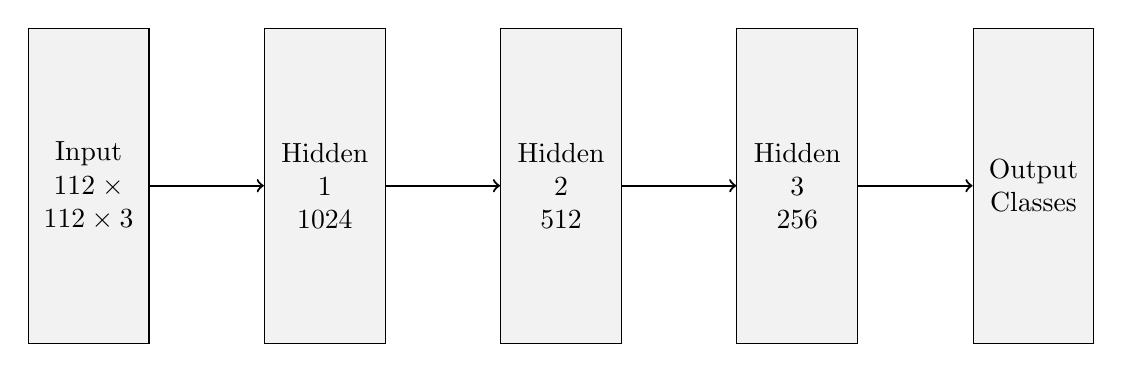
\begin{tikzpicture}[
    node distance = 1.5cm,
    layer/.style = {rectangle, draw, minimum width=1.5cm, minimum height=4cm, fill=gray!10, text width=1.3cm, align=center}
]
    \node[layer] (input) at (0,0) {Input \\ $112 \times 112 \times 3$};
    \node[layer] (h1) at (3,0) {Hidden 1 \\ 1024};
    \node[layer] (h2) at (6,0) {Hidden 2 \\ 512};
    \node[layer] (h3) at (9,0) {Hidden 3 \\ 256};
    \node[layer] (output) at (12,0) {Output \\ Classes};
    \draw[->, thick] (input) -- (h1);
    \draw[->, thick] (h1) -- (h2);
    \draw[->, thick] (h2) -- (h3);
    \draw[->, thick] (h3) -- (output);
\end{tikzpicture}
\caption{Vanilla DNN Architecture}
\end{figure}

\subsection{Self-Taught Learning (STL) with Autoencoder}
A two-stage stacked autoencoder for unsupervised feature learning, followed by supervised classification. This approach helps the model learn compressed, discriminative features.

\begin{figure}[htbp]
\centering
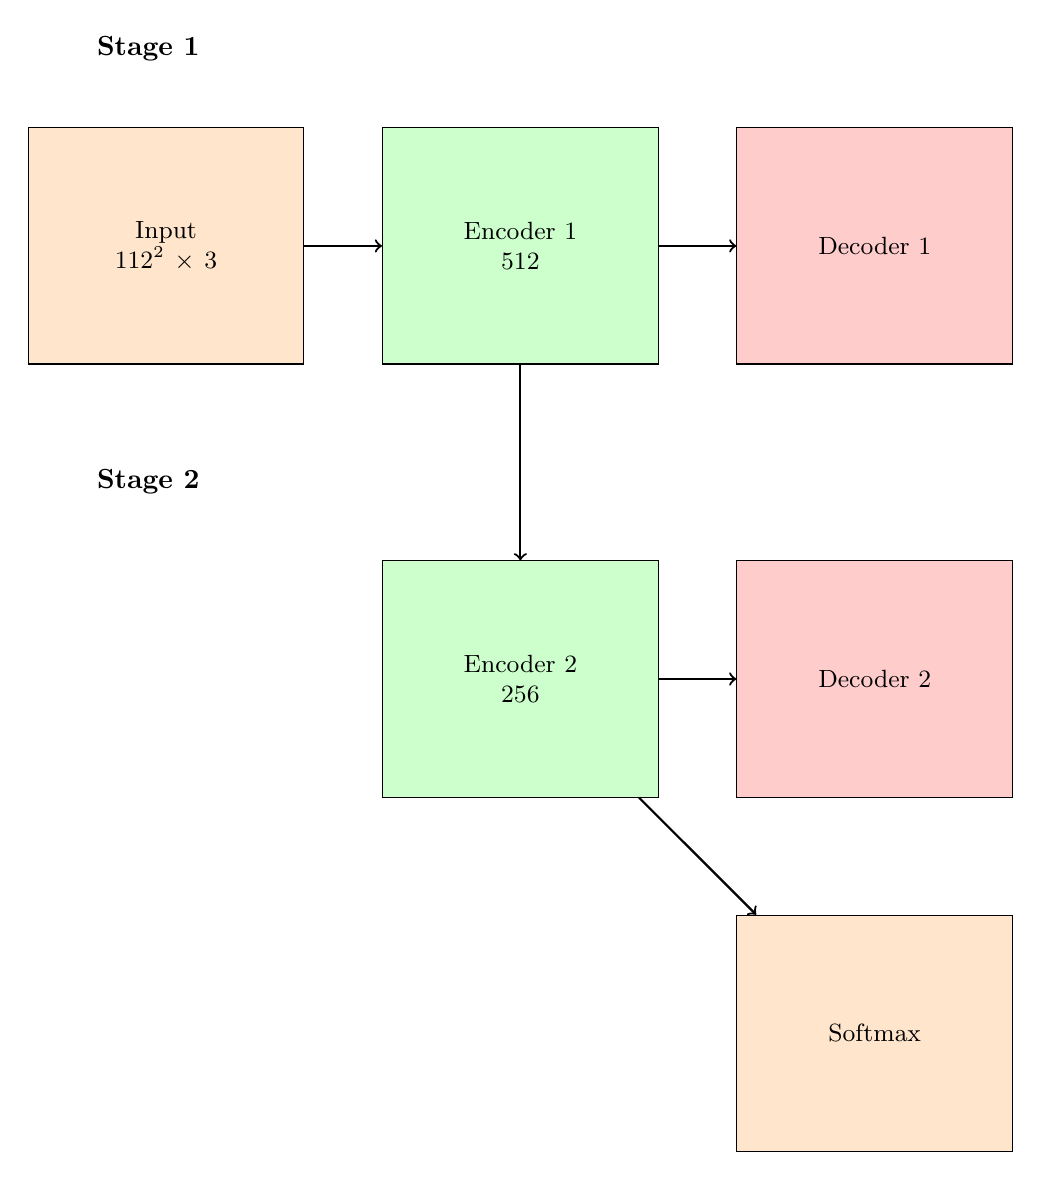
\begin{tikzpicture}[
    node distance = 4.5cm,
    layer/.style = {rectangle, draw, minimum width=3.5cm, minimum height=3cm, fill=orange!20, text width=3.2cm, align=center, font=\small},
    encoder/.style = {rectangle, draw, minimum width=3.5cm, minimum height=3cm, fill=green!20, text width=3.2cm, align=center, font=\small},
    decoder/.style = {rectangle, draw, minimum width=3.5cm, minimum height=3cm, fill=red!20, text width=3.2cm, align=center, font=\small}
]
    % Stage labels moved higher
    \node[font=\bfseries, anchor=west] (title1) at (-1,8) {Stage 1};
    \node[layer] (input1) at (0,5.5) {Input \\ $112^2 \times 3$};
    \node[encoder] (enc1) at (4.5,5.5) {Encoder 1 \\ 512};
    \node[decoder] (dec1) at (9,5.5) {Decoder 1};
    \node[font=\bfseries, anchor=west] (title2) at (-1,2.5) {Stage 2};
    \node[encoder] (enc2) at (4.5,0) {Encoder 2 \\ 256};
    \node[decoder] (dec2) at (9,0) {Decoder 2};
    \node[layer] (classifier) at (9,-4.5) {Softmax};
    % Arrows
    \draw[->, thick] (input1) -- (enc1);
    \draw[->, thick] (enc1) -- (dec1);
    \draw[->, thick] (enc1) -- (enc2);
    \draw[->, thick] (enc2) -- (dec2);
    \draw[->, thick] (enc2) -- (classifier);
\end{tikzpicture}
\caption{Stacked Autoencoder STL Architecture}
\end{figure}

\subsection{Ensemble: SE-ResNet-50 + MobileFaceNet}
Combines two complementary models to leverage both high accuracy and efficiency. The ensemble uses weighted predictions for robust results.

\begin{figure}[htbp]
\centering
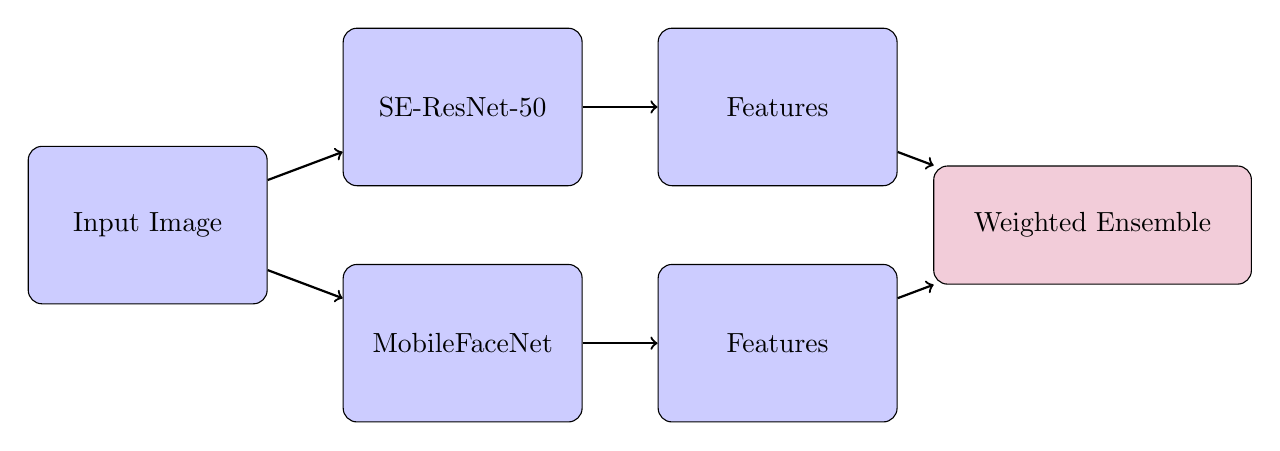
\begin{tikzpicture}[
    node distance = 1.5cm,
    model/.style = {rectangle, draw, minimum width=3cm, minimum height=2cm, fill=blue!20, rounded corners=5pt, text width=2.8cm, align=center},
    ensemble/.style = {rectangle, draw, minimum width=4cm, minimum height=1.5cm, fill=purple!20, rounded corners=5pt, text width=3.8cm, align=center},
    arrow/.style = {->, thick}
]
    \node[model] (input) at (0,0) {Input Image};
    \node[model] (resnet) at (4,1.5) {SE-ResNet-50};
    \node[model] (mobile) at (4,-1.5) {MobileFaceNet};
    \node[model] (feat1) at (8,1.5) {Features};
    \node[model] (feat2) at (8,-1.5) {Features};
    \node[ensemble] (ensemble) at (12,0) {Weighted Ensemble};
    \draw[arrow] (input) -- (resnet);
    \draw[arrow] (input) -- (mobile);
    \draw[arrow] (resnet) -- (feat1);
    \draw[arrow] (mobile) -- (feat2);
    \draw[arrow] (feat1) -- (ensemble);
    \draw[arrow] (feat2) -- (ensemble);
\end{tikzpicture}
\caption{Ensemble Architecture}
\end{figure}

\section{Performance Results}

\begin{table}[htbp]
\centering
\caption{Model Performance Comparison}
\label{tab:perf1}
\begin{tabular}{@{}lcccc@{}}
\toprule
Model & TAR@FAR=$10^{-4}$ & Rank-1 Acc. & Params & Inference (ms) \\
\midrule
Vanilla DNN & 0.742 & 0.835 & 2.1M & 2 \\
Autoencoder STL & 0.833 & 0.884 & 1.8M & 3 \\
SE-ResNet-50 & 0.850 & 0.910 & 23.5M & 15 \\
MobileFaceNet & 0.835 & 0.905 & 0.99M & 3 \\
Ensemble & 0.862 & 0.914 & 24.5M & 18 \\
\bottomrule
\end{tabular}
\end{table}

\begin{table}[htbp]
\centering
\caption{Ensemble + ArcFace Results}
\label{tab:perf2}
\begin{tabular}{lcccc}
\toprule
Model & Accuracy & Precision & Recall & F-Measure \\
\midrule
Ensemble+ArcFace & 0.9186 & 0.9381 & 0.9072 & 0.9224 \\
\bottomrule
\end{tabular}
\end{table}

\end{document}
